Die folgende Grammatik für einfache englische Sätze verwendet
als Terminalsymbole die Wörter
\[
\Sigma
=
\{
\texttt{john},
\texttt{girl},
\texttt{car},
\texttt{saw},
\texttt{walks},
\texttt{in},
\texttt{the},
\texttt{a}
\}.
\]
Die Regeln der Grammatik sind
\begin{align*}
\\
S&\to N'\, V'
& V'&\to V\, N'
& V &\to \texttt{saw}
\\
  &\to N\, V'
  &&\to V\, N
  &&\to \texttt{walks}
\\
  &\to N'\, V
  &&\to V'\, P'
\\
 &\to N\, V
\\
  &
  &N'&\to D\, N
  &N &\to \texttt{john}
\\
  &&
  &\to N'\,P'
  &&\to \texttt{girl}
\\
  &
  &&\to N\, P'
  &&\to \texttt{car}
\\
\\
  &
  &P'&\to P\,N'
  &P&\to \texttt{in}
\\
  &
  &&\to P\, N
\\
  &
  &&
  &D&\to \texttt{the}
\\
  &
  &&
  &&\to \texttt{a}
\end{align*}
\begin{teilaufgaben}
\item
Bringen Sie die
Grammatik in Chomsky-Normalform.
\item
Finden Sie zwei verschiedene Parse Trees für den Satz
\begin{center}
\texttt{john saw the girl in a car}
\end{center}
\item Was ist der Bedeutungsunterschied zwischen den beiden Parse Trees?
\end{teilaufgaben}
Diese Aufgabe zeigt, dass die genaue Bedeutung des Satzes aus der
syntaktischen Analyse alleine nicht erschlossen werden kann.
Zusätzlicher Kontext ist nötig, um die beiden Parse Trees zu unterscheiden.
Dies illustriert, dass maschinelles Verstehen einer natürlichen
Sprache ein nicht triviales Problem ist.

\begin{loesung}
\begin{teilaufgaben}
\item
Die Grammatik hat bereits Chomsky-Normalform,
denn sie enthält nur Regeln der From $A\to BC$, oder $A\to\texttt{a}$
für Terminalsymbole, die Startvariable und das leere Wort $\varepsilon$
kommen nirgends auf der rechten Seite vor.
\item
Bei der Aufstellung der Parse Trees kann man verwenden, dass die unterste
Ebene der Parse Trees durch die Terminalsymbolregeln bereits eindeutig
festgelegt ist.
Auch lässt sich die Kombinationen $DN$ nur aus $N'$ ableiten.
Damit sind die unteren Ebenen des Parse Trees bis zu dem Wort
$NVN'P'$
bereits festgelegt, weiter unten in {\color{blue}blau} dargestellt.

Die Regel $S\to NV$ darf man aber zur Produktion der ersten beiden Variablen
verwenden, denn damit wäre der Satz schon fertig. 
Man muss also entscheiden, ob man mit einer Regel $VN'$ oder $N'P'$
produzieren will.
Beides ist möglich und führt auf die folgenden beiden Parse Trees:
\begin{center}

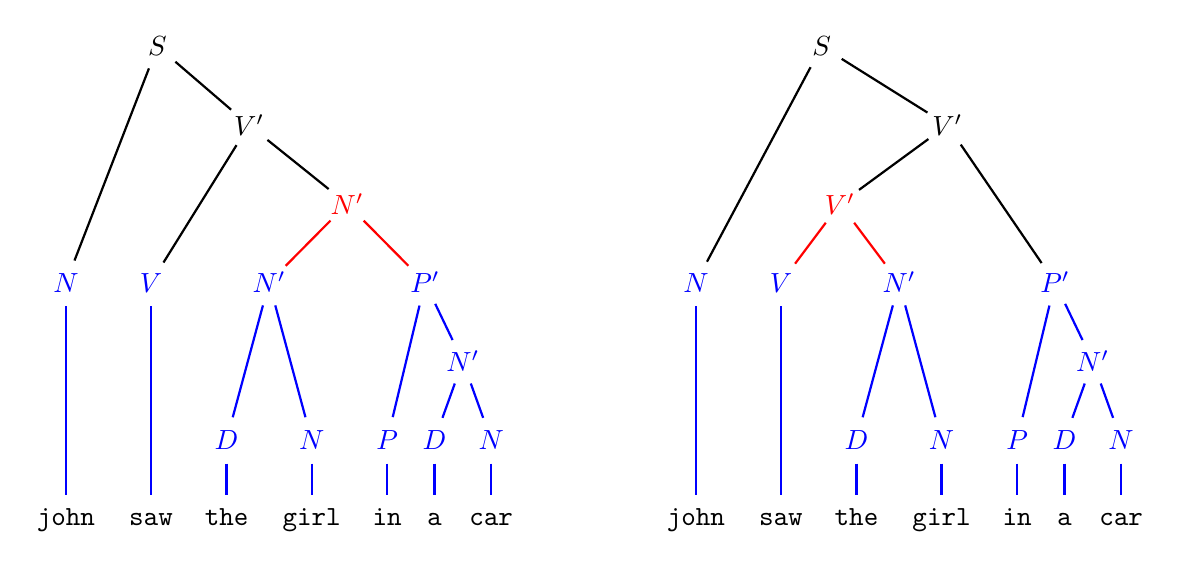
\begin{tikzpicture}[>=latex,thick]

\def\xa{-2.8}
\def\xstep{0.24}
\pgfmathparse{\xa+4.5*\xstep}
\xdef\xb{\pgfmathresult}
\pgfmathparse{\xb+4*\xstep}
\xdef\xc{\pgfmathresult}
\pgfmathparse{\xc+4.5*\xstep}
\xdef\xd{\pgfmathresult}
\pgfmathparse{\xd+4*\xstep}
\xdef\xe{\pgfmathresult}
\pgfmathparse{\xe+2.5*\xstep}
\xdef\xf{\pgfmathresult}
\pgfmathparse{\xf+3*\xstep}
\xdef\xg{\pgfmathresult}

\begin{scope}

\pgfmathparse{0.5*(\xf+\xg)}
\xdef\yf{\pgfmathresult}

\pgfmathparse{0.5*(\xe+\yf)}
\xdef\ye{\pgfmathresult}

\pgfmathparse{0.5*(\xc+\xd)}
\xdef\yd{\pgfmathresult}

\pgfmathparse{0.5*(\yd+\ye)}
\xdef\yc{\pgfmathresult}

\pgfmathparse{0.5*(\xb+\yc)}
\xdef\yb{\pgfmathresult}

\pgfmathparse{0.5*(\yb+\xa)}
\xdef\ya{\pgfmathresult}

\coordinate (A) at (\ya,0);   % ya

\coordinate (B1) at (\xa,-1);
\coordinate (B2) at (\yb,-1); % yb

\coordinate (C1) at (\xa,-3);
\coordinate (C2) at (\xb,-3);
\coordinate (C3) at (\yc,-2); % yc

\coordinate (D1) at (\yd,-3); % yd
\coordinate (D2) at (\ye,-3); % ye

\coordinate (E1) at (\xc,-5);
\coordinate (E2) at (\xd,-5);
\coordinate (E3) at (\xe,-5);
\coordinate (E4) at (\yf,-4); % yf

\coordinate (F1) at (\xf,-5);
\coordinate (F2) at (\xg,-5);

\coordinate (G1) at (\xa,-6);
\coordinate (G2) at (\xb,-6);
\coordinate (G3) at (\xc,-6);
\coordinate (G4) at (\xd,-6);
\coordinate (G5) at (\xe,-6);
\coordinate (G6) at (\xf,-6);
\coordinate (G7) at (\xg,-6);

\node at (A) {$S$};
%\draw[shorten >= 0.3cm,shorten <= 0.3cm] (A) -- (B1);
\draw[shorten >= 0.3cm,shorten <= 0.3cm] (A) -- (C1);
\draw[shorten >= 0.3cm,shorten <= 0.3cm] (A) -- (B2);

%\node at (B1) {$N'$};
\node at (B2) {$V'$};
%\draw[shorten >= 0.3cm,shorten <= 0.3cm] (B1) -- (C1);
\draw[shorten >= 0.3cm,shorten <= 0.3cm] (B2) -- (C2);
\draw[shorten >= 0.3cm,shorten <= 0.3cm] (B2) -- (C3);

\node[color=blue] at (C1) {$N$};
\node[color=blue] at (C2) {$V$};
\node[color=red] at (C3) {$N'$};
\draw[shorten >= 0.3cm,shorten <= 0.3cm,color=blue] (C1) -- (G1);
\draw[shorten >= 0.3cm,shorten <= 0.3cm,color=blue] (C2) -- (G2);
\draw[shorten >= 0.3cm,shorten <= 0.3cm,color=red] (C3) -- (D1);
\draw[shorten >= 0.3cm,shorten <= 0.3cm,color=red] (C3) -- (D2);

\node[color=blue] at (D1) {$N'$};
\node[color=blue] at (D2) {$P'$};
\draw[shorten >= 0.3cm,shorten <= 0.3cm,color=blue] (D1) -- (E1);
\draw[shorten >= 0.3cm,shorten <= 0.3cm,color=blue] (D1) -- (E2);
\draw[shorten >= 0.3cm,shorten <= 0.3cm,color=blue] (D2) -- (E3);
\draw[shorten >= 0.3cm,shorten <= 0.3cm,color=blue] (D2) -- (E4);

\node[color=blue] at (E1) {$D$};
\node[color=blue] at (E2) {$N$};
\node[color=blue] at (E3) {$P$};
\node[color=blue] at (E4) {$N'$};
\draw[shorten >= 0.3cm,shorten <= 0.3cm,color=blue] (E1) -- (G3);
\draw[shorten >= 0.3cm,shorten <= 0.3cm,color=blue] (E2) -- (G4);
\draw[shorten >= 0.3cm,shorten <= 0.3cm,color=blue] (E3) -- (G5);
\draw[shorten >= 0.3cm,shorten <= 0.3cm,color=blue] (E4) -- (F1);
\draw[shorten >= 0.3cm,shorten <= 0.3cm,color=blue] (E4) -- (F2);

\node[color=blue] at (F1) {$D$};
\node[color=blue] at (F2) {$N$};
\draw[shorten >= 0.3cm,shorten <= 0.3cm,color=blue] (F1) -- (G6);
\draw[shorten >= 0.3cm,shorten <= 0.3cm,color=blue] (F2) -- (G7);

\node at (G1) {\texttt{john}\strut};
\node at (G2) {\texttt{saw}\strut};
\node at (G3) {\texttt{the}\strut};
\node at (G4) {\texttt{girl}\strut};
\node at (G5) {\texttt{in}\strut};
\node at (G6) {\texttt{a}\strut};
\node at (G7) {\texttt{car}\strut};

\end{scope}

\begin{scope}[xshift=8cm]

\pgfmathparse{0.5*(\xf+\xg)}
\xdef\yf{\pgfmathresult}

\pgfmathparse{0.5*(\xc+\xd)}
\xdef\ye{\pgfmathresult}

\pgfmathparse{0.5*(\xe+\yf)}
\xdef\yd{\pgfmathresult}

\pgfmathparse{0.5*(\xb+\ye)}
\xdef\yc{\pgfmathresult}

\pgfmathparse{0.5*(\yc+\yd)}
\xdef\yb{\pgfmathresult}

\pgfmathparse{0.5*(\xa+\yb)}
\xdef\ya{\pgfmathresult}

\coordinate (A) at (\ya,0);   % ya

\coordinate (B1) at (\xa,-1);
\coordinate (B2) at (\yb,-1);

\coordinate (C1) at (\xa,-3);
\coordinate (C2) at (\yc,-2);
\coordinate (C3) at (\yd,-3);

\coordinate (D1) at (\xb,-3);
\coordinate (D2) at (\ye,-3);
\coordinate (D3) at (\xe,-5);
\coordinate (D4) at (\yf,-4);

\coordinate (E1) at (\xc,-5);
\coordinate (E2) at (\xd,-5);
\coordinate (E3) at (\xf,-5);
\coordinate (E4) at (\xg,-5);

\coordinate (G1) at (\xa,-6);
\coordinate (G2) at (\xb,-6);
\coordinate (G3) at (\xc,-6);
\coordinate (G4) at (\xd,-6);
\coordinate (G5) at (\xe,-6);
\coordinate (G6) at (\xf,-6);
\coordinate (G7) at (\xg,-6);

\node at (A) {$S$};
%\draw[shorten >= 0.3cm,shorten <= 0.3cm] (A) -- (B1);
\draw[shorten >= 0.3cm,shorten <= 0.3cm] (A) -- (C1);
\draw[shorten >= 0.3cm,shorten <= 0.3cm] (A) -- (B2);

%\node at (B1) {$N'$};
\node at (B2) {$V'$};
%\draw[shorten >= 0.3cm,shorten <= 0.3cm] (B1) -- (C1);
\draw[shorten >= 0.3cm,shorten <= 0.3cm] (B2) -- (C2);
\draw[shorten >= 0.3cm,shorten <= 0.3cm] (B2) -- (C3);

\node[color=blue] at (C1) {$N$};
\draw[shorten >= 0.3cm,shorten <= 0.3cm,color=blue] (C1) -- (G1);
\node[color=red] at (C2) {$V'$};
\node[color=blue] at (C3) {$P'$};
\draw[shorten >= 0.3cm,shorten <= 0.3cm,color=red] (C2) -- (D1);
\draw[shorten >= 0.3cm,shorten <= 0.3cm,color=red] (C2) -- (D2);
\draw[shorten >= 0.3cm,shorten <= 0.3cm,color=blue] (C3) -- (D3);
\draw[shorten >= 0.3cm,shorten <= 0.3cm,color=blue] (C3) -- (D4);

\node[color=blue] at (D1) {$V$};
\draw[shorten >= 0.3cm,shorten <= 0.3cm,color=blue] (D1) -- (G2);
\node[color=blue] at (D2) {$N'$};
\node[color=blue] at (D3) {$P$};
\draw[shorten >= 0.3cm,shorten <= 0.3cm,color=blue] (D3) -- (G5);
\node[color=blue] at (D4) {$N'$};
\draw[shorten >= 0.3cm,shorten <= 0.3cm,color=blue] (D2) -- (E1);
\draw[shorten >= 0.3cm,shorten <= 0.3cm,color=blue] (D2) -- (E2);
\draw[shorten >= 0.3cm,shorten <= 0.3cm,color=blue] (D4) -- (E3);
\draw[shorten >= 0.3cm,shorten <= 0.3cm,color=blue] (D4) -- (E4);

\node[color=blue] at (E1) {$D$};
\draw[shorten >= 0.3cm,shorten <= 0.3cm,color=blue] (E1) -- (G3);
\node[color=blue] at (E2) {$N$};
\draw[shorten >= 0.3cm,shorten <= 0.3cm,color=blue] (E2) -- (G4);
\node[color=blue] at (E3) {$D$};
\draw[shorten >= 0.3cm,shorten <= 0.3cm,color=blue] (E3) -- (G6);
\node[color=blue] at (E4) {$N$};
\draw[shorten >= 0.3cm,shorten <= 0.3cm,color=blue] (E4) -- (G7);

\node at (G1) {\texttt{john}\strut};
\node at (G2) {\texttt{saw}\strut};
\node at (G3) {\texttt{the}\strut};
\node at (G4) {\texttt{girl}\strut};
\node at (G5) {\texttt{in}\strut};
\node at (G6) {\texttt{a}\strut};
\node at (G7) {\texttt{car}\strut};

\end{scope}

\end{tikzpicture}
\end{center}
Die Wahlmöglichkeit, die zu den beiden Parse Trees geführt hat, ist
{\color{red}rot}
hervorgehoben.
\item
Im linken Parse Tree gehört der Teil \texttt{in a car} zu dem
\texttt{girl}, das gesehen worden ist, die Bedeutung ist also, dass
das \texttt{girl} sich im \texttt{car} befunden hat.
Im rechten Parse Tree dagegen beschreibt der Teil \texttt{in a car}
die Tätigkeit von \texttt{john} näher, er sass also im \texttt{car}, als
er das \texttt{girl} gesehen hat.
\qedhere
\end{teilaufgaben}
\end{loesung}

\begin{bewertung}
\begin{teilaufgaben}
\item
Chomsky-Normalform ({\bf C}) 1 Punkt,
Begründung ({\bf B}) 1 Punkt.
\item
Parse Trees ({\bf P}) 3 Punkte.
\item
Bedeutungsunterschied ({\bf U}) 1 Punkt.
\end{teilaufgaben}
\end{bewertung}
